\section{Approach}
\label{sec:Approach}

In this research, we try to tackle the challenges in the context of autonomous manipulation of articulated objects. This section presents the proposed contribution with the goal to fill the gaps in the current research and advance state of the art in this fascinating field. In the previous section, we highlighted the importance of a tight perception and planning framework that can work in close loop. A solution to robust manipulation of articulated objects consists of perception and control algorithms designed to work together. In fact, providing the planner with a more flexible scene representation could help it to come up with better plans. As an example, consider planning in free space. Representing the scene as a signed distance field helps to find collision-free trajectories using the gradient information as opposite to a raw point cloud~\cite{oleynikova2017voxblox}. We want to take the same approach and look at the manipulation problem as the problem of optimizing perception, modeling and planning and their interfaces as a whole, in order to achieve better performance. We envision that the next generation manipulation robots should require little supervision and be robust under different scenario. We hypothesize that the overall framework should contain the following components:
\begin{itemize}
\item \textbf{closed-loop planning}: planning in closed loop has the advantage to incorporate tcurrent (improving) knowledge about the surrounding environment.
\item \textbf{physics-aware planning}: reasoning about all contacts and interactions with the object of interest is of fundamental importance as it does not restrict the motion to high level actions such as push, pull and the grasp to a rigid model.
\item \textbf{expressive scene representation}: the perceptive system should provide interaction-centric information as this facilitates planning and state estimation.
\item \textbf{active uncertainty reduction}: the system can use all its sensing modalities and interaction to better estimate the object model and its parameters. 
\end{itemize}
The development, improvement and implementation of these components is the challenge faced in this thesis. 

\subsection{Assumptions} 

While we want to keep the approach as general as possible, we make a set of assumptions to ameliorate the complexity of the problem:  
\begin{itemize}
\item articulated objects are \textbf{rigid} and belong to the class of open loop kinematic chains consisting of a combination of \textbf{revolute} and/or \textbf{prismatic joints}: we observe that most of the furniture found in household and industrial environments belong to this category.  
\item access to the \textbf{object prior}: we assume that a perception pipeline which provides a reasonable prior about the articulated object is already available. For instance, the algorithm can provide a rough estimate of the joint's location and type (revolute vs prismatic). 
\item manipulation can be solved in a \textbf{non-prehensile} manner: grasp planning is a big research field by its own which has focused prominently on fixed grasps. We make the observation that articulated objects do not necessitate a fixed grasp, especially if the gripper facilitates non-prehesile manipulation as in figure \ref{fig:hook_gripper} 
\item sensing modalities are \textbf{RGB-D images}, \textbf{point clouds}, \textbf{proprioceptive data} and \textbf{wrist-mounted wrench} measurements: these sensors are a standard \emph{de facto} in the robotic community as they are either easy to integrate and/or lots of software tools have been developed for them.
\end{itemize}

\begin{figure}[h!]
    \centering
    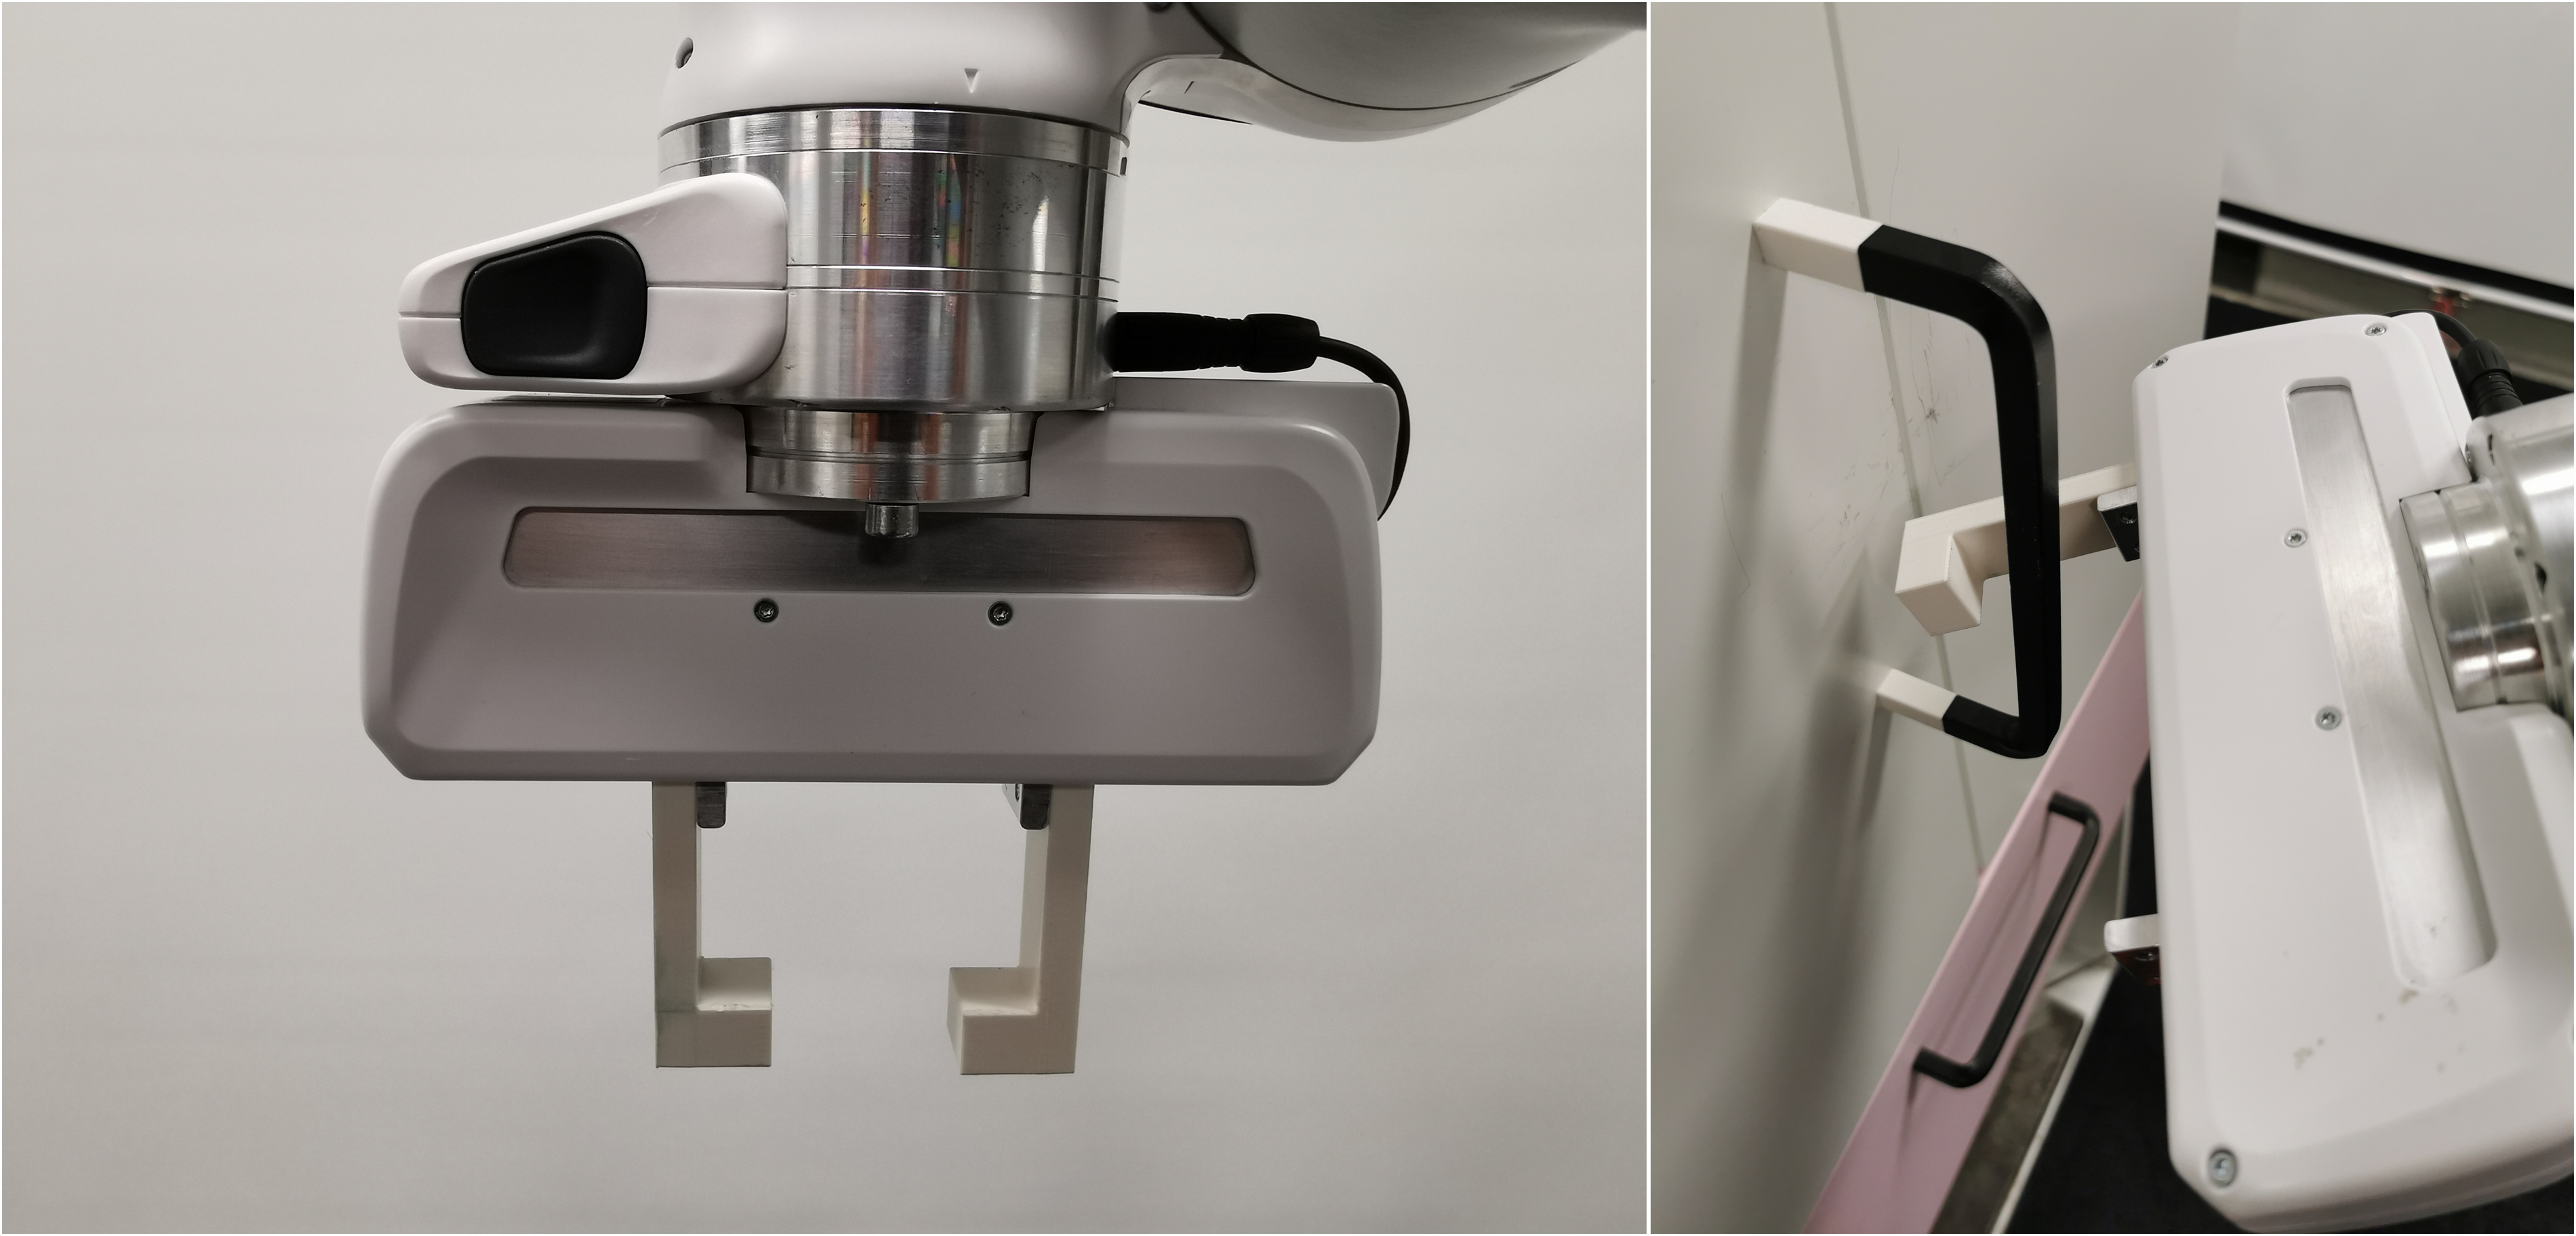
\includegraphics[width=0.4\textwidth]{images/fingers_collage.png}
    \caption{A simple yet effective gripper design can help the manipulation task in a non prehensile setting as the one depicted in figure \ref{fig:dishwasher_handle}}.
    \label{fig:hook_gripper}
\end{figure}

We think that this set of simplifications does not hinder the overarching goal to perform integrated perception and manipulation. Instead we do not make assumptions which are often found in the related literature. We do not have access to human demonstrations, do not rely on a fixed grasp model and a database of high level actions. The scene dynamics is not simplified and motion is not restricted to the plane. Also, the articulated object is not necessarily shaped for easy interactions (e.g. simple graspable handle). 

\subsection{Modules}
The proposed approach is grounded on a powerful gradient-free planning and control method that can sample locally optimal action sequences in complex cost landscapes and complex non differentiable dynamics. Sampling is performed in a simulated twin of the real environment. This planning scheme paves the way to complex vision based cost maps and physical reasoning. We can leverage these features to bridge perception and manipulation planning via an affordance-based costmap. Affordances inform the planner on \emph{interaction hotspots}, namely points where interaction is likely successful and how the interaction is likely to succeed. This source of information complement the local nature of the sampling-based method. Furthermore, as the manipulator moves the perceptual stream changes and so the map derived from it. Consequently perception and planning are coupled in a closed loop fashion. Affordances, on the other hand, can also be interpreted as describing highly informative interaction points as they excite the object motion~\cite{eppner2018physics}. These property can be leveraged to efficiently collect data when the model of the articulated object is not accurately known. Affordances, as well as the cost map they produce, can then be extended to include perceptive uncertainty so that planning can exploit this additional information. The collected visual and haptic data can be compared against multiple simulated scenario to improve the hypothesis about the model's parameters. The improved knowledge about the object can then be dynamically changed in the simulation back-end used for continuous planning. 

\begin{table}[h!]
\hspace*{-1.0cm}
    \begin{tabular}{l|l|l}
     \multicolumn{1}{c}{\emph{Goal}} & \multicolumn{1}{c}{\emph{Sub-topic}} & \multicolumn{1}{c}{\emph{Features}} \\
     \hline \hline
     Interact with known object & Stochastic Control & \textbullet\ Multi-contact interaction \\
                                &                    & \textbullet\ No fixed grasp \\
                                &                    & \textbullet\ Non differentiable cost and dynamics \\   
                                &                    & \textbullet\ Long horizon \\
     \hline
     How and where to interact & Affordances & \textbullet\ Dense interaction-rich representation \\
     with known object         &             & \textbullet\ Dynamic representation \\
                               &             & \textbullet\ Good handling of occlusions \\
     \hline
     How and where to interact  & Multi-scenario & \textbullet\ No quasi-static/planar motion \\
     with partially known object & simulation    & \textbullet\ No high level actions \\
                                &                & \textbullet\ Physical reasoning \\
    \end{tabular}
    \caption{The proposed method is composed of a combination of integrated perception, planning and model estimation modules.}
    \label{tab:modules_table}
\end{table}

% \begin{figure}[h]
% \centering
% 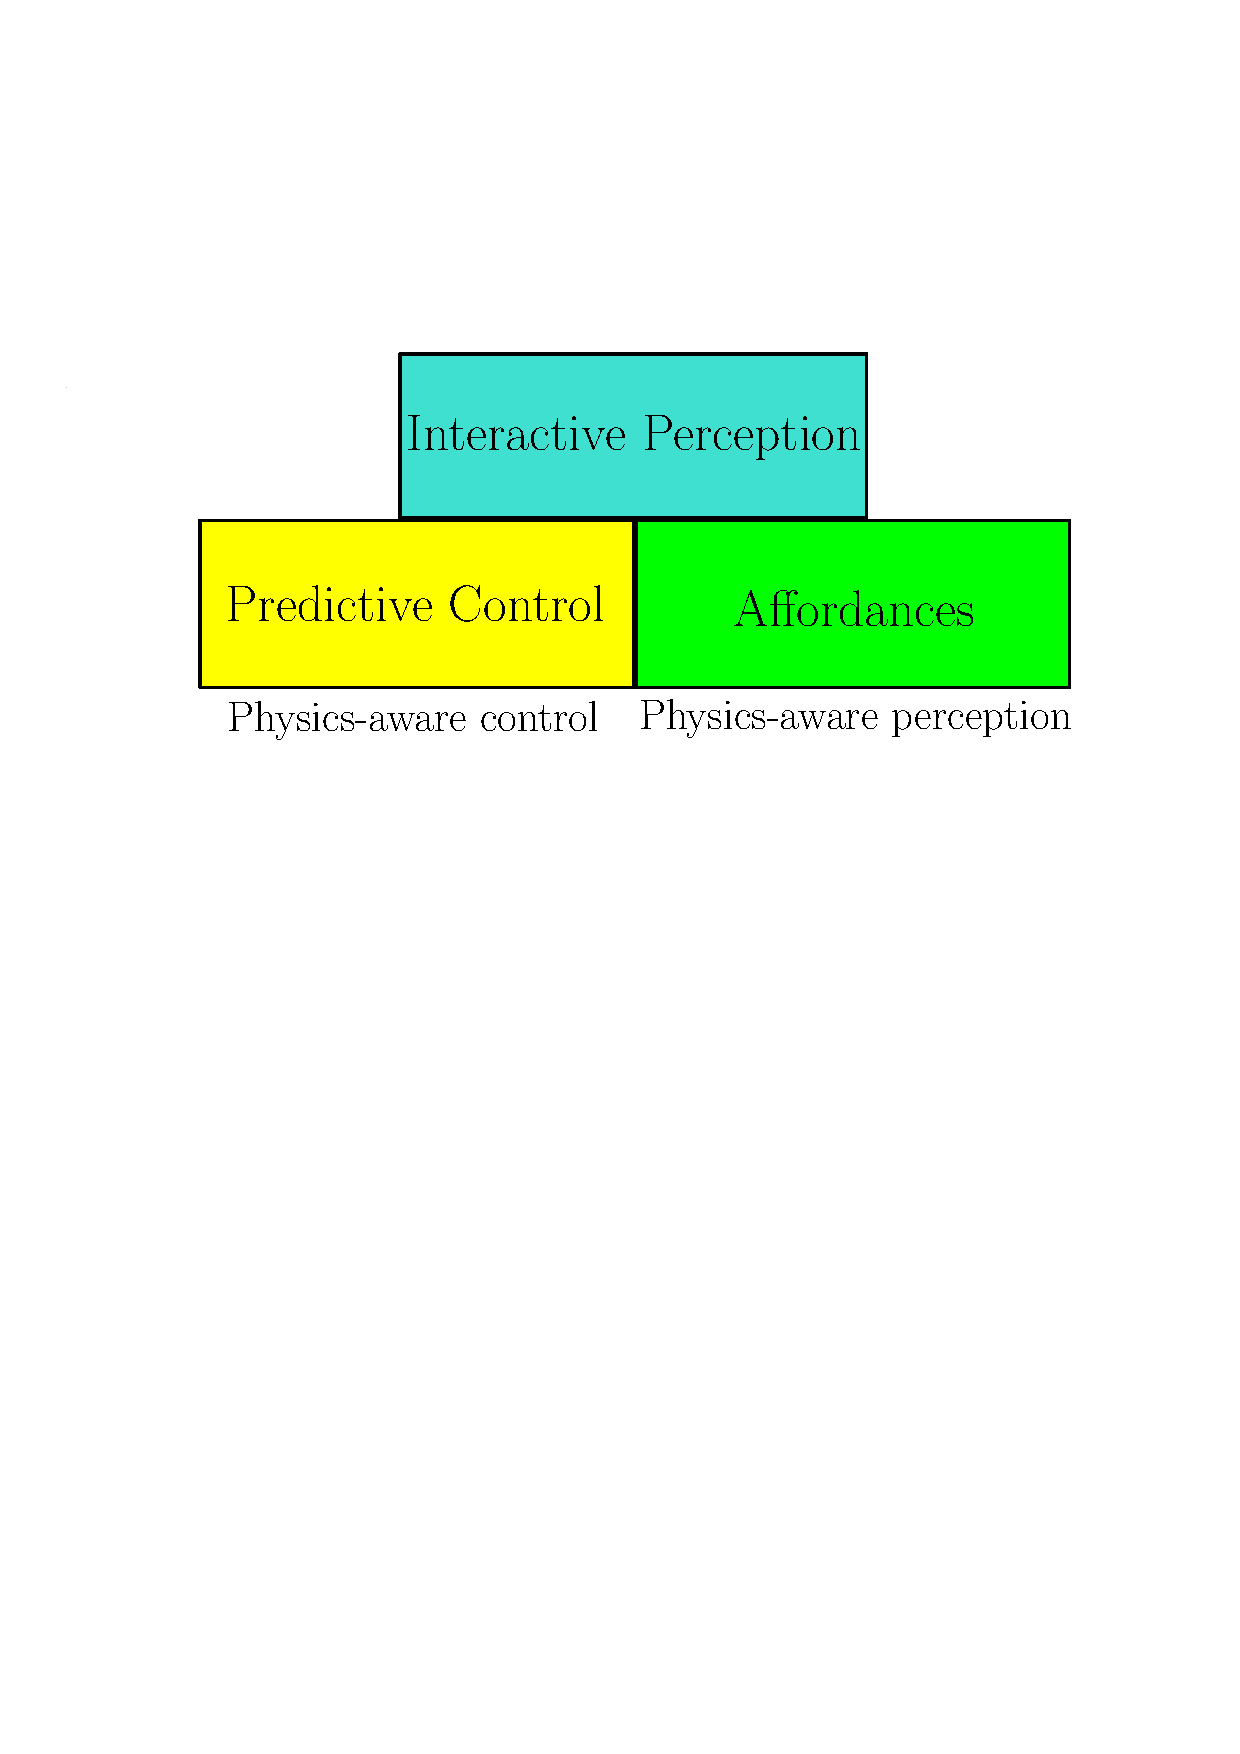
\includegraphics[width=0.6\textwidth]{images/blocks.pdf}
% \caption{Building blocks of the proposed approach: \ldots}
% \end{figure}

\subsubsection{Stochastic Control}\label{sec:pred_control}
The literature generally distinguishes between planning and control algorithms. Here we consider planning as the process of generating a reference signal that the robot can track and brings the system's state (robot and object) to the desired one. For instance, the plan could consist of the robot's joints position and velocity trajectory. These of course are directly related to a corresponding end effector trajectory through forward kinematics. The trajectory is generated such that some objective is optimized, e.g. pulling the door open via interaction. For this task we deploy sampling based methods, as described in section ~\ref{sec:Related Work}. Using a fully fledged simulation back-end is used to sample interaction outcomes. This exploits the fact that basic physical concepts (e.g., distinct objects cannot occupy the same space, gravity applies mass-dependent force on objects, friction and kinematic constraints) are embed in the simulator. Looked from this perspective, our focus is closer to what the literature has often referenced as planning rather then control. 
Nevertheless, the niche of related work that has tried to solve planning through sampling in simulation, has given this methodology the name of \emph{stochastic control}. For coherence with the related work, we will adhere to this nomenclature. Once this reference signal is generated, a \emph{low-level} controller acting at the joint level, converts desired velocities into actual actuator commands. For instance, joints' velocities, can be tracked by a PD controller which ultimately commands joint torques. This computation happens at a fixed rate, so to account for a change in the cost function, external disturbances and the environment. For instance, the robot might need to reach the door handle which is continuously detected by some perception pipeline. In the controller, the cost function penalizes the distance from the end effector to the handle. As the end effector gets closer to the handle, perception might improve, providing a better estimate of the handle's pose and consequently changing the cost used for selecting good samples. In general a cascaded control architecture can be used where the outer loop stochastic controller generates a reference trajectory (e.g. joints' velocities, acceleration or torques) which are then tracked by a low-level controller (e.g. PD, inverse dynamics).  
As shown in the previous example, the cost function is then used as a proxy to inform the controller about the completeness of the task. 
Directly optimizing such a cost in the robot action space is extremely complex. In fact, the mapping between the optimization variables and the cost is highly non-linear. The mapping goes through the full whole-body dynamics and switching interactions that happen between the robot and the articulated object. In this case, the power of traditional optimization methods fall short as accessing the gradient information is complex or not feasible. For this reason, we resort to this class gradient-free methods. 

\paragraph{Research gap and relation to previous works}  This work is based on Model Predictive Path Integral control (MPPI)~\cite{williams_information_2017}, which is the underlying sampling-based controller for whole-body coordination and control. Despite featured with no differentiability requirements, sampling-based methods can be costly to execute and the solution quality is highly dependent on sampling quality. Previous works argue that thousands of trajectories need to be sampled in real time for the effectiveness of the proposed sampling-based algorithm and therefore GPU-based simulation is needed for fast parallel computation~\cite{williams_model_2017}. Unfortunately, GPUs are not common on mobile robots (e.g., because of limited power and payload) and the overall computation times are often not adequate for feedback control. 
Furthermore, demonstrated solutions for tasks involving different physical interactions (e.g. a robot arm opening a drawer~\cite{abraham_model-based_2020}) have been shown on a real system only by breaking down the multi-contact task into stages and enforcing constraints when switching between them. 
This can limit the control envelope of the system and sacrifices solution optimality. For example, it is common practice to fix the gripper orientation between successive reach and pull stages and perform manipulation under a rigid grasp. In the presence of uncertainty and tracking errors, this often leads to high contact forces that might damage the robot as well as the manipulated object.
Ultimately, because of the lack of practical implemented solutions, sampling-based control methods are yet to be applied on real mobile manipulators for whole-body control of complex multi-contact tasks.   

With this prelimiary work we want to verify the following hypothesis:
\begin{displayquote}
\textit{Gradient-free methods enable real-time reactive whole-body mobile manipulation for multi-contact interaction with articulated objects on a real platform with limited computational resources.}
\end{displayquote}

\paragraph{Results} A practical receding horizon algorithm that achieves real-time whole-body control of a mobile manipulator using only a laptop CPU is proposed. We developed several algorithmic elements that enable the controller to achieve performant results, often requiring fewer than 100 rollouts. The main contribution is a regularization of our sampling exploration by means of a momentum update. In fact sampling rollouts can be seen as approximating a gradient descent in a receding horizon fashion~\cite{lambert_stein_2020}. Then momentum regularization, similarly to what is done for static optimization, can be used to trade off the step size and convergence speed. The Raisim physics engine is used for fast and accurate simulation~\cite{raisim} while the Pinocchio library~\cite{pinocchioweb} is used for rigid body dynamics modeling. The developed algorithm is able to control a complex system in real-time without the need for massive parallel computation. To demonstrate the applicability and effectiveness of this approach, several ablation studies are performed in simulation on kinematic and dynamic manipulators. The full algorithm is then deployed on the RoyalPanda platform for a target reaching and door opening task. An open source implementation of the solution is readily available at \url{https://git.io/Jtda7}. The results support the original hypothesis and encourage the deployment of the algorithm to more challenging systems such as aerial manipulators.

\subsubsection{Affordances}
As mentioned in the previous section, control requires the definition of a cost function to know which states are closer to the target state, namely discriminate between bad and good samples. In practice, the true objective is to manipulate the object to a target configuration but we do not care too much about the intermediate robot and object states. The cost then is generally well engineered to encode some prior knowledge of \emph{how} the task should be solved. This prior might not be needed or even be subpotimal for the specific manipulation problem. Consider the running example of opening a door. A high level automaton is often deployed to switch between several cost functions. A initial one for reaching the handle and a second, triggered when the handle is reached and grasped, for keeping the end effector parallel to the handle and opening the door~\cite{abraham_model-based_2020}. We observe that the final objective (door being opened) can be achieved in several different ways. For example one could grasp the handle or apply a pull force to the door edges (if the door is not locked and edges are reachable) and by no means the grasp should necessary stay closed or parallel to the handle. Instead, we could remove the need for a highly engineered cost and let instead behaviors naturally emerge from sampling. In order to cope with the local nature of sampling methods we still need some global interaction-aware representation of the scene. We propose to use then \emph{affordances} to generate a cost map for the controller, a map informing the controller about interesting interaction regions.

\paragraph{Research gap and relation to previous works} The concept of affordances for manipulation has been explored in many recent perception works. They mainly differ in the representation of objects' affordances as interaction points~\cite{gao2021kpam}, interaction regions~\cite{nagarajan2019grounded} or dense interaction likelihood and orientation maps~\cite{mo2021where2act}. Most of these works do not highlight the importance and applicability of the resulting perception pipeline for manipulation control. Furthermore, an agreement on what is the optimal representation of affordances for object manipulation is still missing. In this part of the research, the aim is to combine affordances with control. The goal of this subtask is to verify the following hypothesis:
\begin{displayquote}
\textit{Affordances improve planning performance (success rate, time to completion) in contrast to interaction priors consisting of task decomposition and engineered cost functions.}
\end{displayquote}
The controller can try to bring the robot close to \emph{high-affordance} points. Note that this task can be hard or even infeasible for traditional gradient-based methods, while the sampling-based algorithm we introduced in section~\ref{sec:pred_control} lends itself well to this objective. 
Furthermore, a novel concept of affordances will be explored by introducing haptic information. Intuitively, human not only know by experience \emph{where} to act on object but also \emph{how}. The latter can be expressed in terms of interaction orientations and expected wrench profiles (e.g. pulling vs pushing force). The goal of this second part of the project is to come up with a new definition of affordances which is more powerful as it also contains haptic information. In this task the SAPIEN simulator will be used since it integrates a comprehensive set of articulated objects normally found in households, provides ground truth segmentation and photo-realistic rendering~\cite{Xiang_2020_SAPIEN}. 

\subsubsection{Interactive Perception}
A fundamental aspect to take into consideration for object manipulation is model estimation and the associated \emph{epistemic uncertainty}, which is the uncertainty about the model parameters. For instance, we might not know the geometrical and physical properties of the object such as size, weight, friction, joint positions and orientations. Furthermore, uncertainty can be extended to other types of scene representations such as keypoints and interaction hotspots. Interactive perception will be investigated to reduce such uncertainty by exploiting the robot's capacity to move sensors in space and changing the environment state.

The concept of affordances developed in the previous section provides useful interaction hints. If we are able to perceive which parts of the object are more likely to be interacted with for manipulation and how (e.g handles, edges, indentations), we are also imposing some prior on the type of the articulated object and vice versa. It is then possible to use affordances as a proxy for \emph{explorative actions}. As an example, assume that the robot does not know if the door belongs to a shelf or a car. On the other hand, it can perceive actionable handles through pulling and pushing type of affordances. This can then be used to guide interaction and therefore collect data about how the specific object moves. In this part of the work the goal is to integrate interaction into the perception process.

Forceful interaction, also known as \emph{perceptive manipulation}~\cite{bohg2017interactive} can be used to generate motion and information-rich signals that validate hypotheses about the articulation model. This validation can be performed in a multitude of simulation scenario which serve as a likelihood model. The plan is to integrate \emph{information seeking} actions in the developed stochastic control and perception framework. The components so far developed will serve as building blocks of a simultaneous estimation and control pipeline which works in a closed-loop fashion. We will then investigate the following research hypothesis:
\begin{displayquote}
\textit{Simulation and affordance-guided manipulation is robust to large model uncertainty during simultaneous execution of the task.} 
\end{displayquote}
The sensor modality used to develop the proposed algorithm will be RGB-D cameras and wrist mounted force torque sensors. End-effector mounted cameras are generally good for passive perception but are unusable during manipulation because of heavy occlusions. Therefore, a shoulder or base mounted camera will be evaluated as additional sensory input.  
 
\paragraph{Research gap and relation to previous works} Object classification and articulation model estimation from visual data has already been addressed in previous works~\cite{he2017mask, li2020category}. Although showing promising results, the error from single-shot detection is still in the order of centimeters. The idea of refining the initial estimate using a physics engine to validate exploratory interactive actions has been investigated in~\cite{eppner2018physics}. However, the proposed method relies on a reactive sampling strategy and human intervention for an accurate initial estimate of the articulation model. Frequently, the grasp model is fixed as well as the action parametrization. These assumptions restrict the type of possible interactions and the generalizability of the approach. Furthermore, methods generally split the problem of task execution and model estimation~\cite{eppner2018physics}. Simultaneous parameter estimation and control has been not fully explored for manipulation tasks and has been only applied to low dimensional systems and low dimensional parameter spaces~\cite{barcelos2021dual}. 

\subsection{Leveraging simulation} We believe that the potential of simulation engines (both for physical interaction and rendering) has not been fully exploited in the current research. Contemporary simulators are fast and accurate enough to replace analytical models while rendering engines afford photo-realistic results. Recent behavioral and computation studies of human physical scene understanding push forward an account that people's judgement are best explained as probabilistic simulations of a realistic, albeit noisy, physics engine~\cite{wu2015galileo}.
Simulators could be exploited more in an online fashion. In fact: 
\begin{itemize}
\item Continuous resets keep the deviation of the simulation from the counterpart real observed state small
\item Can update the internal simulation model parameters based on online estimates
\item Detection algorithms can directly act in a virtually rendered scene of the current simulated environment reducing the \emph{sim-to-real} gap.
\end{itemize}
On the other hand, rendering and simulation can be computationally expensive if soft body simulation, detection between complex collision meshes and advanced ray-tracing techniques are deployed. Therefore it is of utmost importance to come up with perception/control methods that require little data by exploiting, for instance, a simplified simulation environment. 

\subsection{Validation} 
During the research project, each component will be evaluated in simulation first and then on the real platform. Simulation will then be used for parameters tuning and fast iteration as well as in order to gain useful insights about the novel approach. In the first part of the project the RoyalPanda mobile manipulator platform will be mainly used for real-world tests and validation. The robot consists of a 7-DoF Franka Emika arm mounted on the holonomic Clearpath Ridgeback base. It offers thus unconstrained workspace which is a key element for successful manipulation. During the project, we will evaluate potential sensors setup as it fits the perception needs. However, we aim to develop a robot agnostic framework that could find potential applications on different platforms, such as aerial manipulators. 